\documentclass[conference]{IEEEtran}
\IEEEoverridecommandlockouts
% The preceding line is only needed to identify funding in the first footnote. If that is unneeded, please comment it out.
\usepackage{cite}
\usepackage{amsmath,amssymb,amsfonts}
\usepackage{graphicx}
\usepackage{textcomp}
\usepackage{xcolor}
\def\BibTeX{{\rm B\kern-.05em{\sc i\kern-.025em b}\kern-.08em
    T\kern-.1667em\lower.7ex\hbox{E}\kern-.125emX}}
\title{
\vspace{1cm}
{
\includegraphics[width=0.15\textwidth]{1.jpg} \\ platformio Assignment} }
\author{AKHILA THALLA\\ Roll No: FWC22312 \\ akhilathalla0104@gmail.com}
 \begin{document}
\maketitle
 \section {ABSTRACT}
 This paper explains the identification of the complete set of logic gates designated as universal gates. Universal gates are logic gates that can implement any Boolean function.
 \section{COMPONENTS}
 The required components list is given in Table:I.,
 \vspace{0.3cm}
 \begin{table} [htbp]
 \centering
 \begin{tabular}{| c | c | c |} \hline
 components & value & quality \\ \hline
 Led's & & 2 \\ \hline
 Arduino & UNO & 1 \\ \hline
 jumperwires & & 50 \\ \hline
 Breadboard & & 1 \\
 \hline
 \end{tabular}
 \vspace{0.3cm}
 \caption{\label{tab:widgets}}
 \end{table}
 \section{PROCEDURE}
 \begin{enumerate}
	 \item Connect the Led's to the Arduino uno.
	 \item Give the inputs manually using jumper wires.
	 \item Truth Table for NAND and NOR gates.
		 \begin{table}[htbp]
			 \centering
			 \begin{tabular}{|c|c|c|c|}
				 \hline
				 A & B & A NOR B & A NAND B \\
				 \hline
				 0 & 0 & 1 & 1 \\
				 \hline
				 0 & 1 & 0 & 1 \\
				 \hline
				 1 & 0 & 0 & 1 \\
				 \hline
				 1 & 1 & 0 & 0 \\
				 \hline
			 \end{tabular}
			 \vspace{0.1cm}
			 \caption{\label{tab:widgets}}
		 \end{table}
	 \item Check the outputs by changing inputs as per truth table.
	 \item Execute the arduino code using the pio run command in nvim editor.
	 \item After upload the code into hardware setup using arduino IDE platform.
 \end{enumerate}
 \section{RESULTS}
 \begin{enumerate}
	 \item Download the code given in the link below and execute them to see the output as shown in Fig.2. 
	 \item https://github.com/Akhilathalla/Akhila/blob/main/platformio/main.cpp                                           
 \end{enumerate}


\begin{figure}[h]                           
\centering                                 
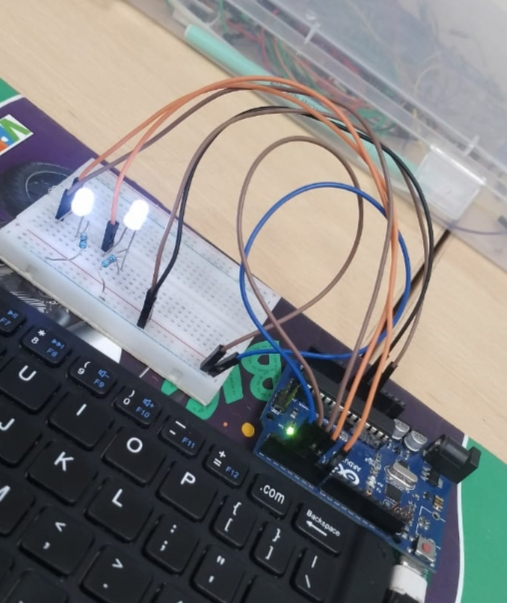
\includegraphics[width=0.4\textwidth]{2.jpg}                                           
\caption{\label{fig-5:Gates}}               
\end{figure}

\section{CONCLUSION}
 Hence implementation of platformio using LED is done and verified through truth table.

 \end{document}

